\chapter{Spark SR1020 Characterization}
\label{cha:characterization}

\section{Introduction}
In this chapter, I will delineate the tests conducted on the Spark SR1020. Initially, I will present the experiments jointly undertaken with Christian Sassi, highlighting personal observations and derived conclusions. Subsequently, I will emphasize the tests specifically targeting power consumption metrics. The objective is to elucidate the methodologies, outcomes, challenges, and findings without revisiting the details already covered in Christian Sassi's dissertation.

\section{Setup and Environment}
All experiments were performed under consistent environmental conditions, ensuring the reliability and reproducibility of results across various settings of the Wireless Core. We strategically elevated the Evaluation Kits (EVKs) using wooden poles to a height of 145 cm to mitigate potential signal reflection from the floor, which could adversely affect performance metrics. The chosen venue for these tests was the West corridor within the Povo 2 building at the University of Trento. This university is renowned for hosting the extensive CLOVES IoT Testbed, a dedicated facility for Ultra-Wideband (UWB) experiments\cite{CLOVES_website}. To minimize external interference, we ensured exclusive access to the testbed and deactivated all other transceivers. However, it's worth noting that certain environmental factors, such as a specific locker's proximity, had a discernible impact on our measurements. The accompanying image illustrates our experimental setup, especially emphasizing the scenario where the receiver board, termed the ‘node’, was adjacent to the aforementioned locker. All conducted tests adhered to a Line Of Sight (LOS) transmission principle.

\begin{figure}[h]
\centering
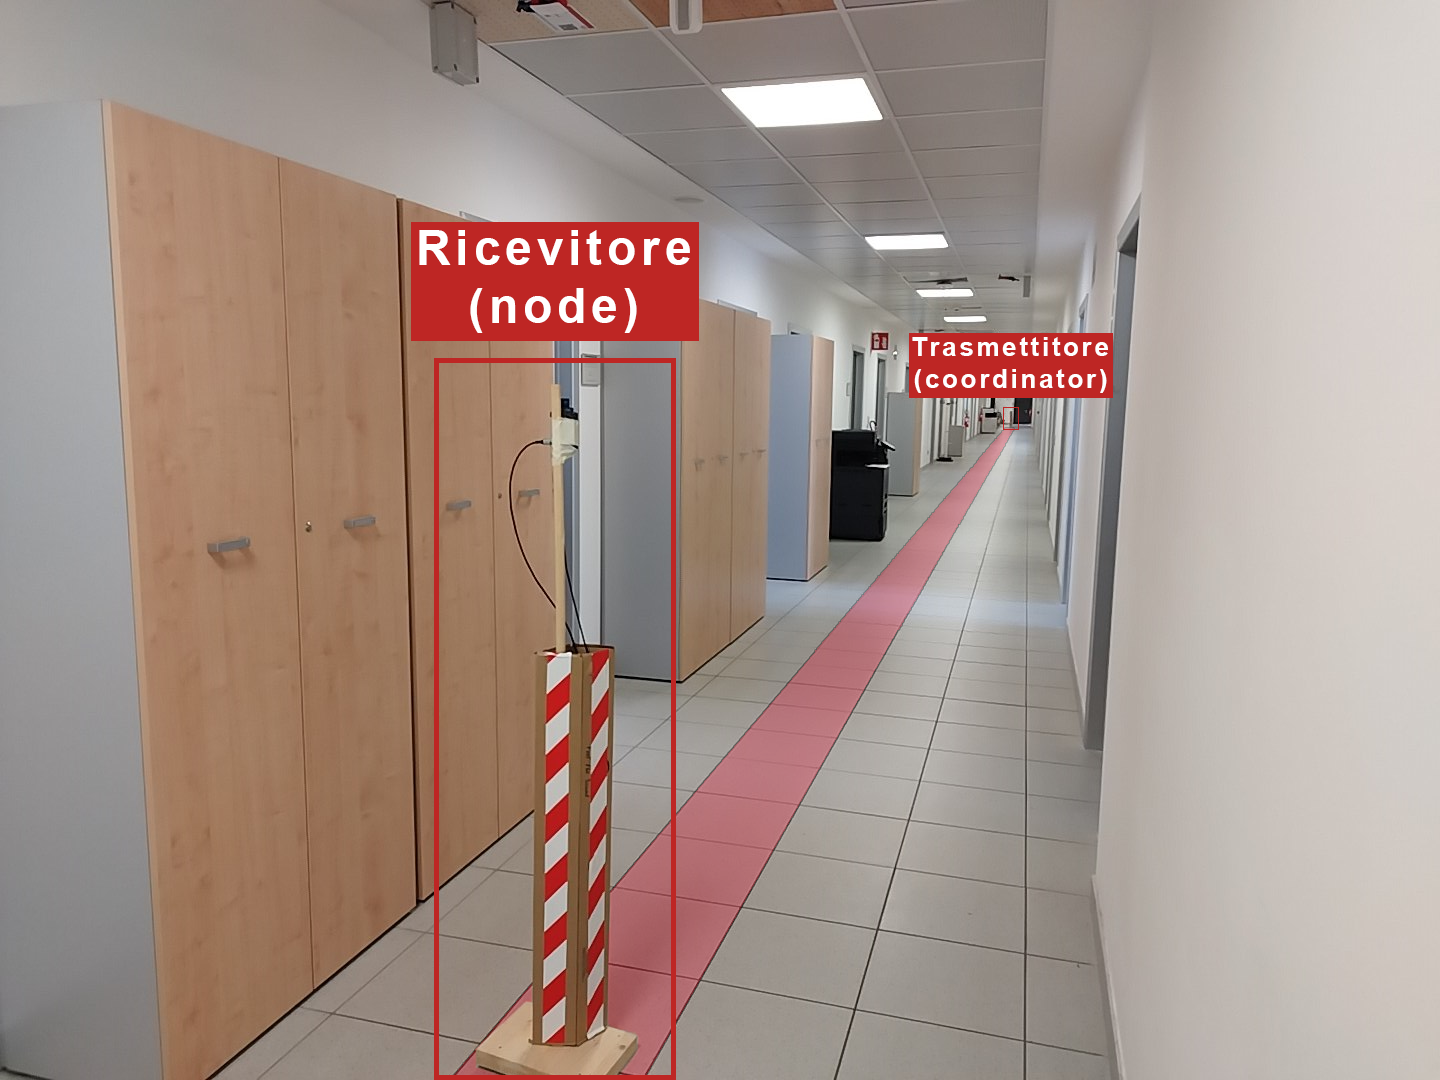
\includegraphics[width=0.8\textwidth]{images/setup test.png}
\caption{Testing Environment}
\label{fig:testing_environment}
\end{figure}

\section{Tests}
Consistency was maintained by employing two distinct boards, designated as ‘node’ and ‘coordinator’ in accordance with Spark's official documentation. Both were configured to execute identical operations. While the 'node' was mobile during tests, the 'coordinator' remained static, serving as our primary connection point. Despite our singular connection to the coordinator, comprehensive statistics for both boards were readily accessible. Given the inherent TDMA-based operation of the Wireless Core, transmissions were scheduled via predefined timeslots. Our experimental paradigm utilized two symmetrical timeslots, each 500 µs in duration, translating to a packet transmission every 1 ms. Features that could potentially introduce variability or unpredictability, such as ARQ, were deliberately disabled. However, we retained the acknowledgment system to effectively monitor the integrity of transmissions.

\subsection{Range Capabilities}
For clarity and precision, I've elected to present only the most robust and pertinent data we amassed. These data points have been consolidated into a single graph presented below. Prior to unpacking the details—especially the noticeable gaps in the 6.5 GHz dataset and the underwhelming performance of the board at this frequency—it's essential to provide context for the data. 
The term 'Coordinator' success rate delineates the Packet Reception Rate (PRR) associated with transmissions originating from the coordinator and directed towards the node. Conversely, the 'Node' success rate signifies the PRR of packets sent by the node to the coordinator. Capturing data from both sources offered deeper insights into the reciprocal transmission behaviors between the radios.
A key observation point was at the 70 m mark, which corresponded to the corridor's terminus, preceding a petite lobby at an intersection of hallways. Tests conducted at 80 m required one board to be placed adjacent to the aisle's terminating wall. This position, within a relatively open expanse, witnessed an uptick in packet reception rates. It is postulated that the wall potentially served as a reflector, enhancing packet reachability to the node. The parameters for these experiments included the Forward Error Correction (FEC) being adjusted to its most minimal setting. This choice was to authentically evaluate range capabilities devoid of augmented payload, which might inadvertently skew power consumption data—a facet I'll explore subsequently.

\begin{figure}[h]
\centering
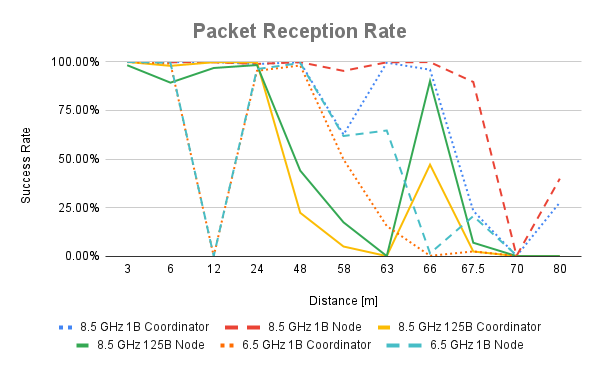
\includegraphics[width=\textwidth]{images/Packet Reception Rate.png}
\caption{Packet Reception Rate}
\label{fig:packet_reception_rate}
\end{figure}


Pivoting to our endeavors at the 6.5 GHz frequency, the results were unfortunately marred by challenges, precluding a full suite of tests akin to the 8.5 GHz frequency trials. Preliminary findings intimate suboptimal performance of radios when operating below 7 GHz, struggling with a limited 6-12 meter range even in ideal conditions. Dedicated tests were carried out to decipher this anomaly. The subsequent graph juxtaposes the success rate in relation to the channel frequency, holding all other variables and the testing environment constant.

\begin{figure}[h]
\centering
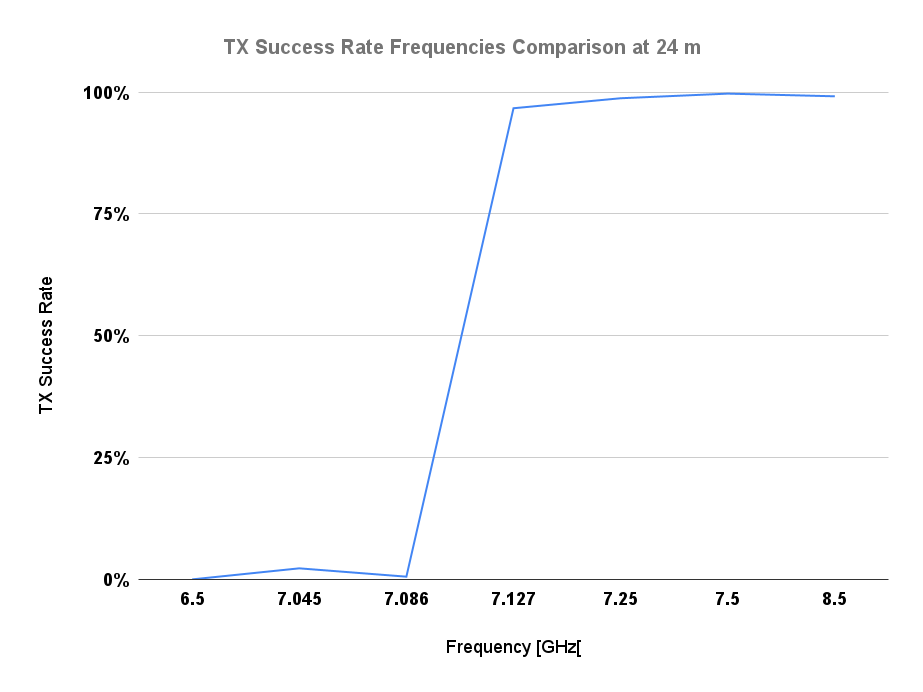
\includegraphics[width=1\textwidth]{images/TX Success Rate Frequencies Comparison at 24 m1.png}
\caption{TX Success Rate Frequency Comparison}
\label{fig:prr_frequency_comparison}
\end{figure}

In the course of my investigation into the underlying causes, I delved into the intricacies of the SDK. Regrettably, due to the lack of support from Spark, I was unable to derive a comprehensive understanding of the phenomena at play. One plausible hypothesis I've formulated is based on Spark's primary application of these radios. Spark predominantly employs these radios for wireless gaming peripherals, encompassing extended reality (XR), headsets, and various gaming devices. Consequently, Spark might have optimized these radios predominantly for short-range scenarios characteristic of such devices.

Subsequent tests were conducted with the Forward Error Correction (FEC) adjusted to the second level. Despite the elevation in the inflation rate to x1.667, the radios exhibited a markedly enhanced performance. Presented below are graphical representations depicting this improved performance and juxtaposing the outcomes from two distinct FEC settings. Additionally, preliminary tests were undertaken with the FEC calibrated to its maximal setting, characterized by an inflation rate of x2. Notwithstanding a marginal improvement in the Packet Reception Rate (PRR), the pronounced inflation rate deleteriously impacted both power consumption and data rate. Hence, our experimental protocol settled on utilizing the second FEC level.

\begin{figure}[h]
\centering
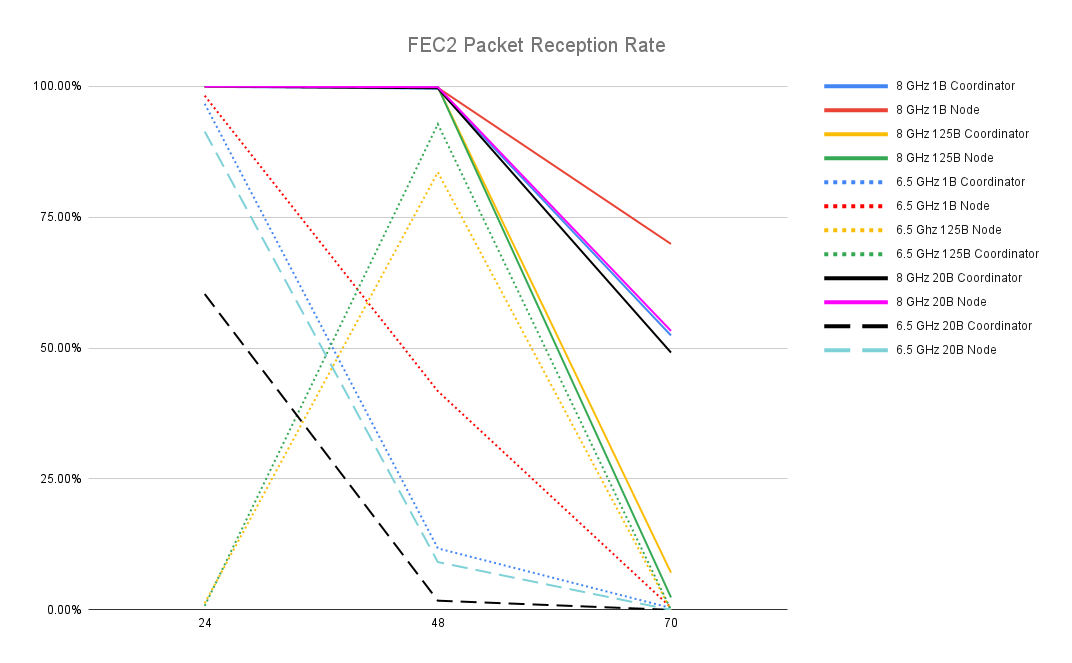
\includegraphics[width=\textwidth]{images/FEC2 Packet Reception Rate.png}
\caption{FEC2 Packet Reception Rate}
\label{fig:fec2_prr}
\end{figure}

A perplexing observation surfaced at the 24m range with FEC 2 and 6.5 GHz: the radios consistently failed to receive any packets. This anomalous behavior persisted across repeated tests, executed at varied intervals and on different days. Notwithstanding our meticulous efforts to mitigate potential interference, the outcome defied our anticipations.

To provide a lucid comparative overview, the subsequent graph delineates the disparity between the two FEC levels. To streamline this representation and given the congruence of the results, only the Coordinator PRR has been plotted, its data being virtually indistinguishable from that of the Node.


\begin{figure}[h]
\centering
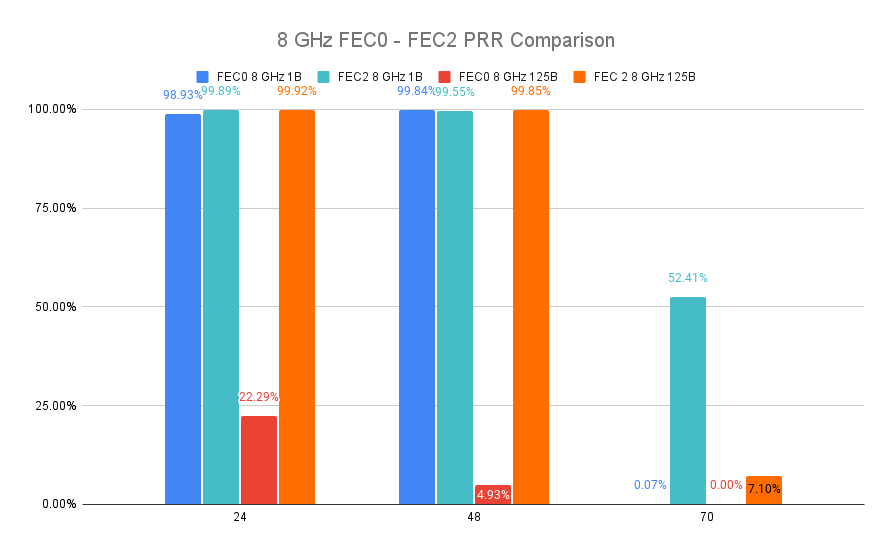
\includegraphics[width=\textwidth]{images/8 GHz FEC0 - FEC2 PRR Comparison.png}
\caption{FEC0 and FEC2 PRR Comparison}
\label{fig:fec0_fec2_comparison}
\end{figure}

\subsection{Power Consumption}
As I will explain in the Challenge chapter, it was infeasible to collect accurate values of power consumption and wake-up timings. I, therefore, decided to report only the data I am confident is correct as I was able to double-check it with different measurement tools. I used the Nordic Semiconductor Power Profiler Kit II (PPK2) and the Diligent Analog Discovery 2. I estimated both metrics based on the data collected and it aligns with what Spark stated. Therefore, I believe that even if for the range capabilities we had some discrepancies between the datasheet and the test results, for what concerns these experiments we did not have many surprises. Figure 3.6 is a Pivot Table that shows the power consumption of the radios using the Idle sleep mode when not communicating.

\begin{figure}[h]
\centering
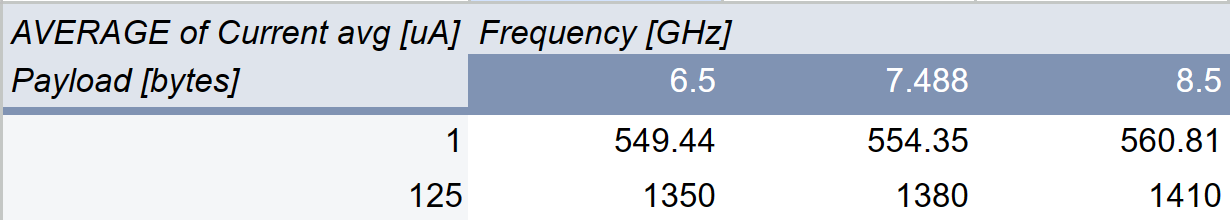
\includegraphics[width=0.8\textwidth]{images/power consumption.png}
\caption{Average Current Pivot Table}
\label{fig:avg_current_pivot}
\end{figure}

Depicted in Figure 4.6 is the average current consumption predicated on the previously described TDMA schedule. A consistent transmission peak, averaging 3.275 mA, was observed throughout the tests. When considering the operational voltage of the radio at 1.8v, its power consumption is discernibly lower, nearly by a factor of ten, when juxtaposed with the DecaWave DW1000, an Ultra-Wideband radio that is in prolific use. This same radio model is also integrated into the University of Trento’s testbed, as discussed in the Setup and Environment section.
%[https://forum.qorvo.com/t/dw1000-power-consumption/10583]

I endeavored to ascertain the delay associated with the wake-up time of all available sleep modes. This necessitated the transmission of impulses via the JTAG expansion connector concurrent with specific occurrences within the event-driven finite state machine intrinsic to the SDK's lower levels. In a corroborative measure, I reduced the TDMA schedule's timeslot duration progressively until the PRR plummeted to 0\%. This strategy aimed at gaining insights into the radio's wake-up latency. Notably, the delays I registered exceeded Spark's official declarations. However, given the methodologies employed, there may have been unavoidable internal delays, thus introducing potential inaccuracies. Figure 4.7 delineates the power states, indicating which devices are active or inactive in each state, accompanied by the respective current usage and wake-up delays.

\begin{figure}[h]
\centering
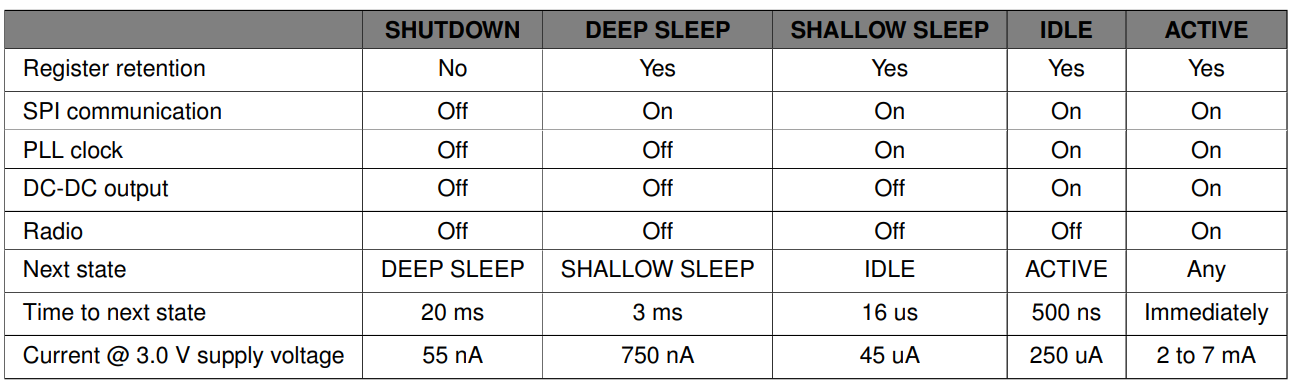
\includegraphics[width=\textwidth]{images/power states datasheet.png}
\caption{SR1020 Power States}
\label{fig:power_states}
\end{figure}


\section{Challenges}
\subsection{Statistics APIs}
Within the Wireless Core architecture, there exists a suite termed 'statistics APIs', dedicated to data extraction from the employed connections. Regrettably, not all the specified functions are fully realized or operational as anticipated. Certain functions, instead of returning values directly, appear to rely on other lower-level functions to update specific structures; this frequently results in absent or incorrect updates. An in-depth probe revealed vestigial functions and structures, possibly remnants from earlier SDK iterations, thus culminating in functional aberrations. Although I managed to retrieve additional values beyond those illustrated in the SDK examples, they fell short of expectations. Consequently, there exists a paucity of data on nuanced metrics such as link quality. However, metrics like RSSI (Received Signal Strength Indicator) and RNSI (Received Noise Strength Indicator) were retrievable. These assisted in demystifying the suboptimal performance of radios at frequencies below 7 GHz. Intriguingly, occasional readings for both metrics registered 0 dB — while conceivable for the RSSI, it's improbable for RNSI due to the ever-present noise factor. Given these inconsistencies, such values were excluded from the characterization.

\subsubsection{Serial Communication}
Data transmission to the boards via serial proved insurmountable despite the presence of relevant functions and the appropriate utilization of the HAL (Hardware Abstraction Layer) within the SDK. Engaging with Spark on this challenge yielded the revelation that this capability has not been extended to the Evaluation Kits. The rationale behind this unilateral serial transmission remains enigmatic to us, but it undeniably curtailed our ability to optimize test execution through automation.

\subsection{Accurate Power Consumption Measurement}
In an effort to derive precise data on power consumption, it became evident that the power profilers utilized were not adept at discerning the distinct stages of the transceivers, such as wake-up, transmission, synchronization, and so forth. When an attempt was made to integrate a shunt resistor between the designated current measurement header pins, an unintended diversion of current was observed, ostensibly from an alternative component of the circuit. This rendered oscilloscope-based measurements impractical.

When a minimal resistance was incorporated for current measurement related to the radio, the oscilloscope predominantly displayed electrical noise. Conversely, slightly increasing this resistance resulted in the current bypassing our intended path and instead traversing another section of the PCB, which left the resistor devoid of any current. Incremental adjustments, even by a single Ohm, failed to produce a satisfactory measurement condition. Notably, this appears to be a slight oversight in the PCB design. Interestingly, this investigative process illuminated the fact that the radios maintained functionality even when the current measurement header pins were entirely disengaged, drawing current entirely from alternative pins. This anomaly was closely studied in collaboration with Davide Molteni, a technician affiliated with the Department of Information Engineering and Computer Science. Our consensus posits that the radio might be sourcing its current through the CS (Chip Select) pin associated with the SPI interface.

From a theoretical standpoint, the optimal approach to executing these tests without altering the hardware might entail employing a sophisticated oscilloscope, equipped with an efficient probe and a shunt positioned between the current measurement pins. Nevertheless, the plausibility of this method remains ambiguous, given the challenges posed by potentially negligible voltage levels susceptible to noise interference. In the event of this approach being untenable, two viable alternatives emerge:

\begin{enumerate}
  \item Extracting the radio from the EVK and subsequently engineering a breakout board that effectively connects the two. This setup would incorporate test pads, current measurement pin headers, and jumper connections across all pins bridging the two PCBs. This configuration promises enhanced insight into the current distribution across the various radio pins.
  \item Rethinking the radio PCB's design from its foundational stage. Commencing with solely the SR10X0 chip and adhering to the hardware design guidelines could prevent such inadvertent current flow patterns. 
\end{enumerate}


%[ADD LINK TO WEB PAGE]

\newpage




